% Appendix B

\chapter{Novel Method to Choose the Best Classifiers} % Main appendix title

\label{AppendixB} % For referencing this appendix elsewhere, use \ref{AppendixA}

\lhead{Appendix B. \emph{Novel Method to Choose the Best Classifiers}} % This is for the header on each page - perhaps a shortened title

It was mentioned in future work, in Chapter \ref{chapter6}, that it would be beneficial if it was possible to identify the top \textit{n} models without having to manually evaluate each separately. The ideas presented here are not necessarily a complete solution. They do, however, represent a possible future line of investigation. Were the ideas suggested here a proven methodology, the model evaluation sections of \ref{chapter5} would have read something like this.

\section{Choosing the Best Classifiers}

Having completed all NLTK and Scikit-Learn modelling, the next task was to identify which models performed the best to be further evaluated using simulation and which models, even though their performance measures are good, are to be discarded. As previously discussed, the criteria to determine the best model was that it should first maximise recall for the positive bullying class and secondly that it must also maximise recall for the negative not bullying class. As discovered in the literature review in Section \ref{section:3.3}, \citet{kubat_addressing_1997} referred to this measure as the geometric mean of the accuracies measured separately on each class or as $g =\sqrt{\frac{TP}{TP + FN} \cdot \frac{TN}{TN + FP}}$, from now on referred to as the \textit{g-performance}. This measure is essentially the square root of the positive class recall multiplied by the negative class recall. Also to be taken into consideration is the nature of any manipulation performed on the data, for example, over sampling or under sampling, and also the run time. With all these factors taken into consideration the top classifiers will be further evaluated in the next section by way of a simulation of live data.

It was decided that the three best models across all evaluation criteria would go forward for further examination.

\subsection{G-Performance}

The first measure evaluated to determine which models were the best was g-performance. The value for each model was calculated and a heat map generated from the results is shown in Figure \ref{fig:best_model_01}. It can clearly be seen that there are six clusters of results that are very similar and that all these clusters represent either over sampling of the minority class or a hybrid sampling approach.

\begin{figure}[htbp]
	\centering
	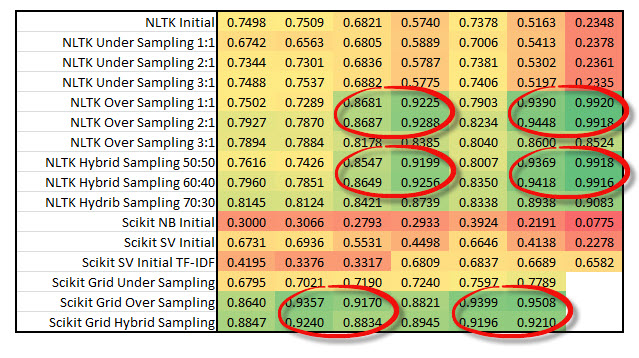
\includegraphics[width=1\textwidth]{Figures/Chapter5/best_model_01.jpg}
	\caption[Best Model - G-Performance heat map]{Heat map showing the g-performance measurement for all models}
	\label{fig:best_model_01}
\end{figure}

\subsection{Execution Time}

The second evaluation criterion was the execution run time of each model. The longest run time was 27.1118 seconds whilst the fastest was 0.727 seconds. Clearly, in their raw format, these numbers are out of proportion with the g-performance measures. To resolve this all times were normalised between 0 and 1. The normalised times were then weighted to reflect, that whilst important, run time is not a deciding factor. A weighting of 0.2 was applied to reflect that the g-performance measurement was 5 times more important than the run time measure. Through examination it was found that below 5, run time was too influential, whilst above 10, it made little impact. Figure \ref{fig:best_model_02} shows the resulting heat map with the fastest and slowest times identified. 

It should be noted that low runtime was considered as positive  implying that 0.2 is representative of the fastest time and 0.0 was the slowest time recorded. What is very clear from the heat map is that Scikit-Learn significantly outperforms the NLTK.

\begin{figure}[htbp]
	\centering
	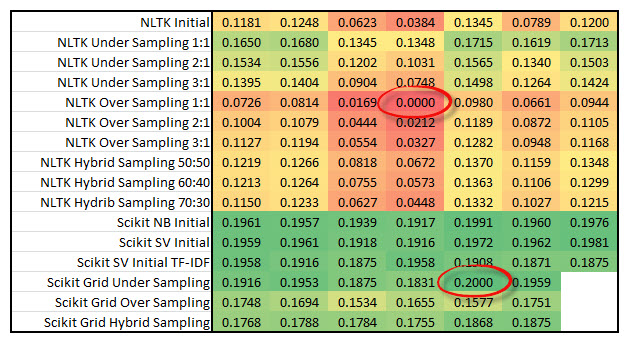
\includegraphics[width=1\textwidth]{Figures/Chapter5/best_model_02.jpg}
	\caption[Best Model - Normalised execution heat map]{Heat map showing the normalised execution run time for all models}
	\label{fig:best_model_02}
\end{figure}

It is unfortunate that the execution times used here include all data reading, data writing, data manipulation and model training times. It would have been ideal if the time taken to predict each sample was available for each model. The reason the prediction time is important, is that generating the model, and all that entails, could be done on a high specification back-end server. If the work described here was deployed on a smart phone, for example, the application would probably only have to predict single samples at a time, using a previously generated model deployed using Pickle. From work in Section \ref{subsection:applying-classifiers}, classification times for a single sample were in the region of 0.0013 seconds for an NLTK model, and 0.000034 seconds for a scikit-learn model. Both of these times are so fast as to suggest that the end user would not notice the difference, making this measurement redundant. However, these times were achieved on a high-end laptop with significantly more processing power than the average smart phone. If this measure was to be included in any novel model evaluation method, the values used would have to be based on actual times from the targeted platform.

\subsection{Data Manipulation}
 
The final evaluation criterion to be considered was the manipulation performed on the data. It was important to acknowledge the fact that the sampling applied directly affects the performance of the model and some counter balance, or penalty, should be applied. Having made the decision that the models where data manipulation was used would be penalised it was decided that the maximum penalty would be 0.1 or that the g-performance was 10 times more important than any data manipulation penalty. Using 0.1 as the maximum value, the different class ratios were penalised as shown in Table \ref{tab:chapter5:ratio_penalty}. The resulting heat map of penalties for all models run is shown in Figure \ref{fig:best_model_03}

\begin{table}[h]
	\centering
	\caption[Penalties assigned for sampling]{Table showing the penalties applied to the various ratios when sampling of data was used}
	\label{tab:chapter5:ratio_penalty}
	\begin{tabular}{ll}
		\toprule
		\textbf{Class Ratio}& \textbf{Penalty}    \\
		\midrule
		3:1 & 0.05   \\
		2:1 & 0.075   \\
		1:1 & 0.1   \\
		70:30 & 0.05   \\
		60:40 & 0.075   \\
		50:50 & 0.1   \\
		None & 0   \\
		\bottomrule
    \end{tabular}
\end{table}

\begin{figure}[htbp]
	\centering
	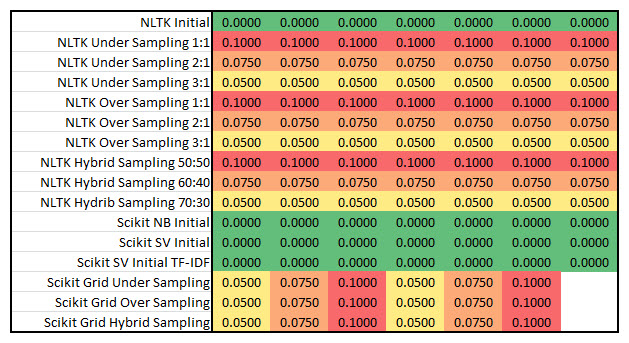
\includegraphics[width=1\textwidth]{Figures/Chapter5/best_model_03.jpg}
	\caption[Best Model - Data Manipulation Penalties]{Heat map showing the penalties applied to each model where sampling of data was involved}
	\label{fig:best_model_03}
\end{figure}

\subsection{Best Models}
The best models were then calculated as \textit{Best Model = Max(G-Performance + Run Time - Ratio Penalty)}. So models with high g-performance but with low run time weighting and low data manipulation penalties will be chosen. The final heat map, identifying the three best models is shown in Figure \ref{fig:best_model_04}. The three models are:

\begin{enumerate}

	\item NLTK Naive Bayes Hybrid Sampling with 60:40 ratio using tri-grams excluding stop words
	\item Scikit-Learn Support Vector Hybrid Sampling with 60:40 ratio using uni-grams and bi-grams including stop words
	\item Scikit-Learn Naive Bayes Over Sampling with 2:1 ratio using uni-grams, bi-grams and tri-grams including stop words

\end{enumerate}

\begin{figure}[htbp]
	\centering
	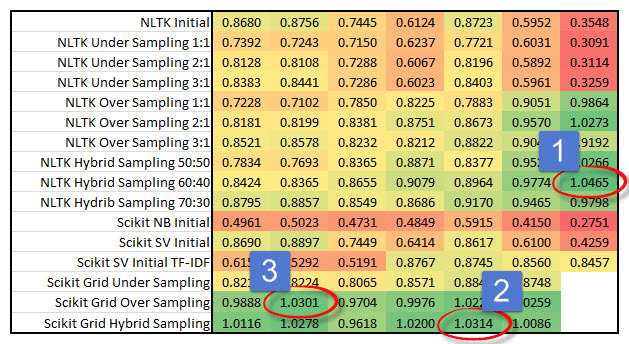
\includegraphics[width=1\textwidth]{Figures/Chapter5/best_model_04.jpg}
	\caption[Best Model - Three best models identified]{Heat map the final results and identifying the best models}
	\label{fig:best_model_04}
\end{figure}

It is clear that under sampling never approached the performance levels of over sampling and hybrid sampling and that the middle sampling ratios always appeared to give more balanced results then the other ratios.

These three models will now be further examined in the next section.

\section{Applying the Best Classifiers}
\label{subsection:applying-classifiers_app}

Now that the best three classifiers have been determined the final analysis task is to determine which of the three perform best in a simulation of a real life scenario. 

\subsection{Scenario Overview}
A classifier is to be developed that will batch process a corpus of previously unseen questions, called \verb|dataset_02|, to determine whether or not they are bullying in nature. The predictions, bullying or not bullying, from each batch of questions processed are then fed back into the training dataset and a new classifier model is generated. The next batch of questions is then classified. This process continues until all sample have been processed. 

A third test dataset, \verb|dataset_03|, never used at any point in the development of any of the classifiers will be used to gauge the performance of each of the models before and after the batch processing in order to determine which model produced the best classifier.

The steps to achieve this can be summarised as follows:

\begin{itemize}

	\item Prepare the two datasets put aside for this testing in Chapter \ref{chapter4} by generating NLTK or Scikit-Learn corpora as required.
	\item Classify both datasets using the three top models and record the performance results.
	\item Simulate the growth in each of the models using \verb|dataset_02|.
	\item Re-evaluate \verb|dataset_03| again using each of the final models and see if the models performance has increased or decreased. Also compare the complete set of before and after results from \verb|dataset_02|.

\end{itemize}

\subsection{Data Preparation}
At the end of Chapter \ref{chapter4} \verb|dataset_02| and \verb|dataset_03| had not been preprocessed or stored in the correct corpora format for NLTK or Scikit-Learn. In a real life scenario, the processing required to do this would all have to happen as the data is received. However, in this simulation all preparatory work was performed upfront. Each dataset was first preprocessed and cleansed using the same Python script as described in Section \ref{section:data_prepatation}. Next, each datasets was saved in the basic NLTK corpus format and renamed as \verb|simulation_01| and \verb|hold_back_01|. The NLTK model that was to be tested required the dataset in tri-gram format with stop words removed producing two further NLTK corpora called \verb|simulation_13| and \verb|hold_back_13|. Both of the Scikit-Learn models used the NLTK \verb|simulation_01| and \verb|hold_back_01| corpora but with all the samples presented in a single comma separated file format as before.


\subsection{Initial Analysis of Models}
Once each dataset had been prepared they were submitted to their respective model for analysis. The results from the two Scikit-Learn models will be discussed shortly but first the performance of the NLTK model is analysed. It was immediately noticed that the number of examples presented to the model was significantly fewer than expected. Also, the performance of the model was very poor in comparison to the performance achieved by the training model.

Originally there were 87,205 and 11,193 samples respectively in the simulation and hold back datasets. However, after processing was applied to these datasets to remove stop words and then convert them to tri-grams, it resulted in only 53,804 and 6,976 samples submitted to the NLTK model. A reduction in sample numbers of approximately 38\%. On analysis, it was clear that the cause of this was the conversion to tri-grams. When a sample question had less than three tokens a tri-gram could not be generated resulting in an empty sting. In a production environment the loss of 38\% of all samples because of a processing step would not be an acceptable  solution.

The other issue with the NLTK model was its predictive performance on the previously unseen data in the simulation and hold back datasets. After manual classification of the training dataset, approximately 17\% of the samples were identified as bullying. After training, the NLTK classifier could nearly identify 100\% of all positive, bullying, and negative, not bullying, samples. Although a classifier is never expected to perform as well on unseen data only 2.5\% of the hold back samples and 2.4\% of the simulation samples were identified as bullying. Although further more detailed analysis would be required to confirm this, a quick review of the tokens in the samples that were identified as bullying suggested that the NLTK model had been over fitted to the training data and did not generalise well to unseen data. 

Based on these finding the NLTK model was dismissed as a viable solution. No further testing using this model was performed.

Because the Scikit-Learn TF-IDF vectorise class also included uni-gram tokens when generating bi-grams of a sample and both uni-grams and bi-grams when generating tri-grams these models did not suffer the same loss of samples that the NLTK model did. The Scikit-Learn hybrid sampling model classified 1,878 of the hold back samples and 14,172 of the simulation samples, equivalent to 16.8\% and 16.3\% respectively, as bullying. These numbers are very consistent with the percentage of bullying samples seen in the training dataset. The over sampling model did not appear to have performed as well identifying 1,128, 10.1\% and 8,752, 10.0\% samples in hold back and simulation datasets. Although not appearing to have performed as well as the hybrid sampling model, it did still appear to have performed consistently across the two datasets.

\subsection{Batch Processing of Samples}

Each Scikit-Learn models was then further examined using the simulation dataset as follows:

\begin{itemize}

	\item The simulation dataset of 87,205 samples was divided into twenty distinct datasets.
	\item Then for each of these datasets:
	
	\begin{itemize}
	
		\item The training dataset was loaded
		\item The training dataset was sampled as required by the model, either hybrid sampling or over sampling
		\item A classifier model was created using the sampled training data
		\item The simulation dataset was classified using the model
		\item The classified simulation samples were appended to the training dataset
		\item Process repeated until there were no further simulation datasets 
	
	\end{itemize}
	
	\item Once all the simulation samples are included in the final model, the hold back dataset was classified and the results were written to a file.

\end{itemize}

This simple process was repeated for hybrid sampling and over sampling. In addition to writing the hold back classification results to file, each of the results for the classification of the simulation samples were also written to file. The results of this batch processing and classification of the hold back data was then analysed.

\subsection{Analysis of Batch Processing Results}
The first thing to note was that the increase in processing time as the size of the training set grew appeared linear. This linearity would make it possible to predict the time required for larger datasets. It was also observed that there was a significant difference between the two different types of sampling used with over sampling taking more time. This difference is probably down to the fact that uni-grams, bi-grams and tri-grams are used with over sampling opposed compared to just uni-grams and bi-grams with hybrid sampling. The processing time results can be seen in Figure \ref{fig:execution_time} starting with the original training dataset of 9,543 samples for the first iteration all the way to 96,748 samples for the last.

\begin{figure}[htbp]
	\centering
	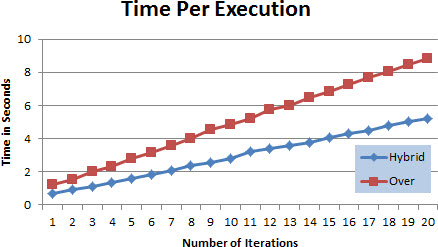
\includegraphics[width=0.75\textwidth]{Figures/Chapter5/execution_time.jpg}
	\caption[Processing time for batch simulation]{Chart plotting the different processing time when batch processing using hybrid and over sampling}
	\label{fig:execution_time}
\end{figure}

The hybrid sampling model was the first to be examined. The initial model developed using only the training dataset predicted 1,878 of the hold back dataset samples as bullying. The model at the completion of the batch processing experiment predicted 2,449 bullying samples. This represents a 30.4\% increase in the number of samples classified as bullying. On closer examination it was seen that of the 1,878 original bullying predictions only 1,685 were again classified as bullying, 193 bullying samples were reclassified as not bullying and 764 not bullying samples were now classified as bullying. 

The over sampling model was then analysed. The initial model developed using only the training dataset predicted 1,128 of the hold back dataset samples as bullying. The model at the completion of the batch processing experiment predicted 1,218 bullying samples. This represents a 8.0\% increase in the number of samples classified as bullying, a much smaller increase than seen with the hybrid sampling classifier. On closer examination it was seen that of the 1,128 original bullying predictions 898 were again classified as bullying, 230 bullying samples were reclassified as not bullying and 320 not bullying samples were now classified as bullying.

As a percentage, just under 90\% of the samples using hybrid sampling were predicted as bullying before and after the batch processing but only 80\% of the over sampling predictions remained the same. Looking at the number of new bullying classifications, as a percentage of the original number, the hybrid sampling was again the better performer at an additional 40.6\% new bullying classifications compared to 28.4\%. Finally, only 10.3\% of samples initially classified as bullying using hybrid sampling were reclassified as not bullying compared to 20.4\%. These would all suggest that the hybrid sampling model performed better by maintaining the highest percentage of predicted bullying samples, by adding a higher percentage of new bullying samples and also by reclassifying fewer bullying samples as not bullying.

It would be impossible, time wise, to re-examine all 11,193 samples in the hold back dataset from both sampling methods so the samples that changed classification were all reviewed and manually classified to determine if any patterns existed in the way samples were reclassified.

Hybrid sampling was analysed first. In total 193 samples changed from bullying to not bullying and 764 changed from not bullying to bullying. Each of the 957 samples, which represents 8.5\% of the total amount, was manually classified as either bullying or not bullying using the criteria defined in Section \ref{section:data_classification}. The percentage of each class that was either correctly or incorrectly reclassified was calculated. The results are shown in Figure \ref{fig:sim_results_02}.

\begin{figure}[htbp]
	\centering
	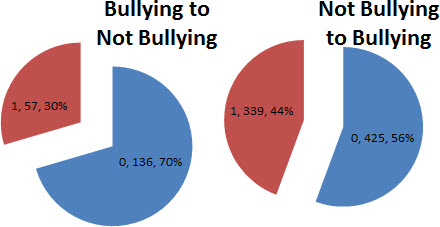
\includegraphics[width=0.75\textwidth]{Figures/Chapter5/sim_results_02.jpg}
	\caption[Analysis of Hybrid Sampling on Hold Back Dataset]{Analysis of hybrid sampling prediction performance on the hold back dataset after batch processing of simulation data}
	\label{fig:sim_results_02}
\end{figure}

Of the 193 samples that were reclassified from bullying to not bullying, shown on the left hand side of Figure \ref{fig:sim_results_02}, it was determined that 136 or 70\% of the samples were incorrectly reclassified and were, in fact, originally correctly classified as bullying. Of the 764 samples that were reclassified as bullying it was seen that 425, 56\%, were correctly reclassified as bullying, but it was also shown that 339 or 44\% of the samples should not have been reclassified.

When the analysis of the over sampling was complete, a similar picture was seen as shown in Figure \ref{fig:sim_results_03}.

\begin{figure}[htbp]
	\centering
	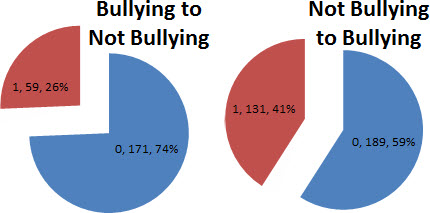
\includegraphics[width=0.75\textwidth]{Figures/Chapter5/sim_results_03.jpg}
	\caption[Analysis of Over Sampling on Hold Back Dataset]{Analysis of over sampling prediction performance on the hold back dataset after batch processing of simulation data}
	\label{fig:sim_results_03}
\end{figure}

On examination of the numbers shown in Figures \ref{fig:sim_results_02} and \ref{fig:sim_results_03} it would appear, when looking past the initial earlier analysis which suggested that hybrid sampling was the better performing model, that neither model appears very stable with a high percentage of incorrect predictions. However, given that an acceptable number of false positives, samples incorrectly predicted as bullying, with a high positive class recall value is the primary criteria to which a model must perform, the hybrid sampling method is clearly the better model.

To complete the analysis of the Scikit-Learn hybrid sampling model, 100 of the 1686 samples predicted as bullying that did not change classification after the batch processing of the additional samples were manually classified. Of the 100 samples, 87\% were correctly classified as bullying. The original model had an positive recall value of 94.9\% so although this recall value is not as good, the overall performance of the Scikit-Learn hybrid sampling model is very satisfactory.
